\section*{Assignment 04: Monetisation Strategy}
\addcontentsline{toc}{section}{Assignment 04: Monetisation Strategy}

This section converts spreadsheet experiments into a monetisation roadmap anchored in platform theory instead of wishful thinking.

\subsection*{Revenue options and theoretical grounding}
I shortlisted four revenue streams and matched each to explicit principles from \citet{Choudary2016} and \citet{HagiuWright2013}.
\begin{itemize}
  \item \textbf{Completion fee.} A seven percent fee only triggers once both sides confirm delivery. Hagiu and Wright argue that transaction fees should align with realised value to avoid discouraging participation, so the fee stays invisible until success is logged.
  \item \textbf{Enablement subscription.} Larger partners can upgrade to a monthly enablement tier that bundles templated briefs, analytics, and advisory sessions. \citet{Choudary2016} lists producer tools as the second monetisation layer once the core interaction works, so this tier waits until the grow phase.
  \item \textbf{Insight reports.} Aggregated skill and impact trends can be sold to universities and municipal innovation teams. \citet{ShapiroVarian1999} note that information goods scale cheaply, yet \citet{Zuboff2019} warns about surveillance, so reports only launch with differential privacy, opt in consent, and the governance checks described in Assignment~05.
  \item \textbf{Grant funded scholarships.} Philanthropic grants and university funds can subsidise stipends for resource constrained NGOs. This follows \citet{ShapiroVarian1999}'s price discrimination guidance and keeps inclusion aligned with Assignment~07's fairness commitments.
\end{itemize}

\subsection*{Sequencing across the lifecycle}
I map timing to the seed, grow, scale arc from \citet{Choudary2016}.
\begin{enumerate}
  \item \textbf{Seed months zero to six.} No fees. The focus is on trust rituals: weekly office hours, concierge onboarding, and a public roadmap. Success means thirty completed projects and satisfaction above four point five.
  \item \textbf{Early grow months seven to twelve.} Introduce the seven percent completion fee for new organisations while grandfathering the founding cohort for three months. Pilot the enablement tier with five agencies and track completion above eighty five percent, churn below ten percent, and net promoter score above plus thirty. These thresholds come from lecture case studies on balancing monetisation with quality \citep{Lecture05}.
  \item \textbf{Scale beyond month twelve.} Extend fees to all partners, roll out enablement broadly, and launch the insight reports once the data board signs off on privacy safeguards. Monitor revenue per active organisation alongside engagement to catch extraction risks \citep{Srnicek2017}.
\end{enumerate}

\subsection*{Experiments and cost discipline}
Each revenue stream carries a paired experiment. The completion fee gets an A B test comparing disclosure at brief creation versus after matching. The enablement tier runs through Van Westendorp pricing interviews with at least twenty organisations; launch only happens if the acceptable range centres between four hundred and five hundred DKK. Insight reports start with a diary study involving fifteen participants who rate trust on a five point scale; anything below three forces a redesign. Costs stay visible: fixed year one spend sits near six hundred twenty thousand DKK for product, design, and operations, while variable costs scale with completed sprints. Break even requires roughly one thousand fifty projects per year, a number pulled from Assignment~09's capacity model.

Figure~\ref{fig:student-profile} shows the student profile interface that makes these revenue streams plausible. It surfaces badges, skill evidence, and mentor quotes that organisations value, while prompts encourage students to keep data fresh. The mock up enacts \citet{Choudary2016}'s advice to monetise after creating tangible producer surplus.

\begin{figure}[H]
  \centering
  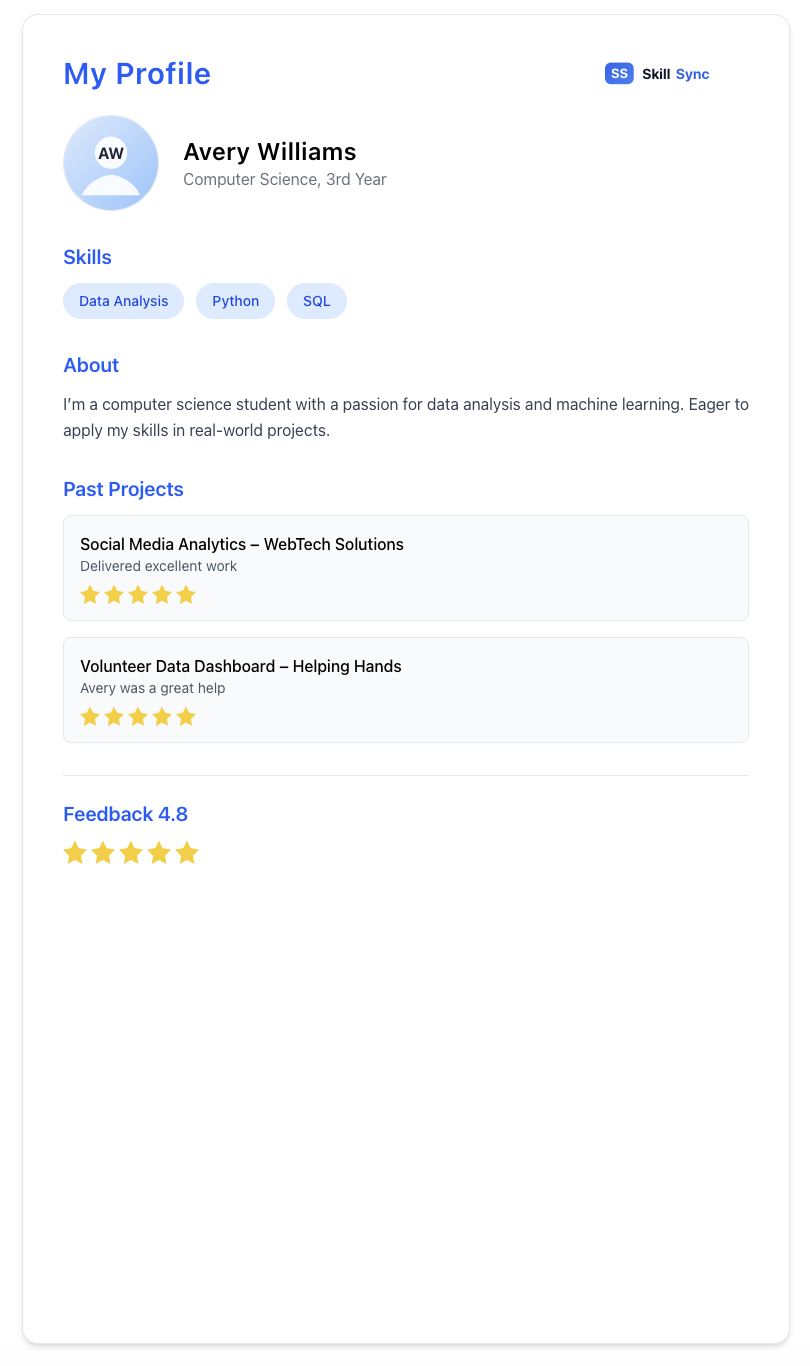
\includegraphics[width=0.8\linewidth]{figures/Student-Profile.png}
  \caption{Student profile mock up highlighting evidence that underpins monetisation.}
  \label{fig:student-profile}
\end{figure}

Ethical guardrails conclude the plan. Insight reports wait until at least five organisations in a sector and five hundred completed projects are available. Consent screens explain why each datapoint is collected, and grants stay separate from transaction fees so subsidies do not distort signals. These safeguards translate \citet{Zuboff2019}'s critique into product requirements.
